% -*- latex -*-
%-----------------------------------------------------------------------
%;  Copyright (C) 2006
%;  Associated Universities, Inc. Washington DC, USA.
%;
%;  This program is free software; you can redistribute it and/or
%;  modify it under the terms of the GNU General Public License as
%;  published by the Free Software Foundation; either version 2 of
%;  the License, or (at your option) any later version.
%;
%;  This program is distributed in the hope that it will be useful,
%;  but WITHOUT ANY WARRANTY; without even the implied warranty of
%;  MERCHANTABILITY or FITNESS FOR A PARTICULAR PURPOSE.  See the
%;  GNU General Public License for more details.
%;
%;  You should have received a copy of the GNU General Public
%;  License along with this program; if not, write to the Free
%;  Software Foundation, Inc., 675 Massachusetts Ave, Cambridge,
%;  MA 02139, USA.
%;
%;  Correspondence concerning AIPS should be addressed as follows:
%;          Internet email: aipsmail@nrao.edu.
%;          Postal address: AIPS Project Office
%;                          National Radio Astronomy Observatory
%;                          520 Edgemont Road
%;                          Charlottesville, VA 22903-2475 USA
%-----------------------------------------------------------------------
%Body of final AIPSletter for 31 December 2005

\documentclass[twoside]{article}
\usepackage{graphics}

\newcommand{\AIPRELEASE}{December 31, 2006}
\newcommand{\AIPVOLUME}{Volume XXVI}
\newcommand{\AIPNUMBER}{Number 2}
\newcommand{\RELEASENAME}{{\tt 31DEC06}}
\newcommand{\OLDNAME}{{\tt 31DEC05}}
\newcommand{\NEWNAME}{{\tt 31DEC07}}

%macros and title page format for the \AIPS\ letter.
\input LET98.MAC

\newcommand{\MYSpace}{-11pt}

\normalstyle

\section{General developments in \AIPS}

\subsection{Current and future releases}

We have formal \AIPS\ releases on an annual basis.  While we offer a
full binary installation method for both the frozen and development
versions for MacIntosh OS/X (PPC and Intel chips), Solaris, and Linux
systems, all architectures can do a full installation from the source
files.  The current release is called \RELEASENAME\ and is now
``frozen.''  If you took a development copy of this version at some
earlier date, you may use the ``Midnight Job'' (MNJ) to bring it up to
date.  You need to run a MNJ only once in 2007 to convert your copy of
\RELEASENAME\ into the frozen version.  When patches to 2006 are
announced, you may apply them with the MNJ\@.  This \Aipsletter\ is
intended to advise you of corrections and improvements in this
release.

We have begun a new version, called \NEWNAME, which is now under
development by the \AIPS\ Group.  You may fetch and install a complete
copy of this version at any time.  Having fetched \NEWNAME, you may
update your installation whenever you want by running the MNJ which
uses cvs, rsync, and transaction files to copy and compile the code
selectively based on the code changes and compilations we have done.
We expect users to take their source-only or binary version of
\NEWNAME\ \AIPS\ over the Internet (via \emph{anonymous} ftp).  Both
versions require you to copy the installation procedure {\tt
install.pl} via {\tt ftp}; the source-only version also requires you
to ftp the 88-Mbyte {\tt \NEWNAME.tar.gz} compressed tar file.

From {\tt mnj.aoc.nrao.edu}, the MNJ will serve up \AIPS\
incrementally --- or as a whole --- using the Unix tool {\tt cvs}
running with anonymous ftp.  Binary MNJs also use the {\tt rsync}
tool.  Linux sites will almost certainly have {\tt cvs} installed;
other sites may have installed it along with other GNU tools.
Secondary MNJs will still be possible using {\tt ssh} or {\tt rcp} or
NFS as with previous releases.  We have found that {\tt cvs} works
very well, although it has one quirk.  If a site modifies a file
locally but in an \AIPS-standard directory, {\tt cvs} will detect
the modification and attempt to reconcile the local version with the
NRAO-supplied version.  This usually produces a file that will not
compile or run as intended.

\AIPS\ is now copyright \copyright\ 1995 through 2007 by Associated
Universities, Inc., NRAO's parent corporation, but may be made freely
available under the terms of the Free Software Foundation's General
Public License (GPL)\@.  This means that User Agreements are no longer
required, that \AIPS\ may be obtained via anonymous ftp without
contacting NRAO, and that the software may be redistributed (and/or
modified), under certain conditions.  The full text of the GPL can be
found in the \texttt{15JUL95} \Aipsletter\ and is included with every
distribution in file {\tt \$AIPS\_ROOT/{\it release-name}/COPYING}\@.
\vfill\eject

\subsection{Installing a new version}

If compiling locally, new releases must be installed from the tar ball
for that release.  If using the binary installation, a full new
installation must also be done with {\tt rsync}.  The {\tt cvs} system
requires this.  When installing a new \AIPS\ release in a system that
already has a previous release, we recommend that {\tt install.pl} be
used and that the previous release be left in place, at least until
the installation has been seen to work.  If you do this, then you will
not have to re-edit the disk, printer, and tape lists and can simply
skip all those pages in the {\tt install.pl} menus.  The old {\tt
  \$HOME/.AIPSRC} file may be left in place, but it will need to be
edited.  The lines giving the {\tt DOWNLOADED} and {\tt UNPACKED}
parameters should be deleted and the {\tt CCOMOPT} line should be
changed to point to the current release rather than the previous one
--- the {\tt -I} parameter really should be {\tt -I\$INC} but it gets
its full path name instead.  This forces a re-edit with each release.
If you have made special versions of {\tt UPDCONFIG} and {\tt
do\_daily.{\it host}}, you should preserve them under new names and
restore them after the install.  If you have an odd set of \AIPS\
versions, the {\tt \$AIPS\_ROOT/AIPSPATH.*SH} files may need to be
edited after the install to set the desired versions.

For Linux, Solaris Ultra, and MacIntosh systems, a binary installation
is available from CDrom, supported by {\tt install.pl}.  Alternatively,
the frozen version may be installed with the binary installation
method now present in {\tt install.pl}.  The ftp site for downloading
files directly has been eliminated.

\section{Binary installations and updates}

GNU has provided compilers for the \AIPS\ community at no cost for
many years.  While remarkably good, these compilers have suffered from
both minor errors and from their generality.  When some vendor sets
out to make a compiler for a very specific architecture, it is
possible --- not guaranteed --- to create a compiler that produces
binaries that run faster than those produced by GNU's {\tt g77}.
Unfortunately, these vendors have to recover their costs in producing
these compilers and so may charge for them at a rate that is difficult
or prohibitive for many \AIPS\ users.  Such is the case with IBM's {\tt
  xlf} compiler for PPC chips, including the MacIntosh OS/X systems,
for SUN's SUNWspro compiler suite, and for Intel's {\tt ifort}
compiler.   These compilers produce executables that run about 50\%\
faster (30\%\ faster for Intel) than those produced by {\tt g77} on
these operating systems and cpus.  Fortunately, their licensing
agreements allow us to ship executables to our users along with the
required run-time libraries.  The binaries produced by the Intel
compiler for Linux are quite large because they contain optimizations
for modern PIV cpus, older PIV cpus, and for general computers such as
AMDs.  The specific optimizations to be used are selected
automatically at run time.

The code to implement the binary installation and binary updates via
the MNJ is comparatively simple.  Every night, a {\tt cron} job run on
the master \AIPS\ machine in Socorro, does the necessary magic to make
the daily cvs snapshot of \AIPS, builds the tar-ball, orders the four
architectures at the AOC to do ordinary text MNJs, and then {\tt
rsync}'s the binaries and text to a special area on the computer used
for public {\tt ftp} access to NRAO in Socorro.  The installation
script must be fetched from the AOC anonymous ftp area to your desired
{\tt \$AIPS\_ROOT} area and then executed with

\begin{center}
\vskip -12pt
{\tt \Large perl install.pl -n}
\vskip -12pt
\end{center}

With the {\tt -n} option, the script will skip fetching and unpacking
the tar-ball and the compiler queries and usage.  It does a variety of
{\tt rsync} commands to fetch a complete copy of the \AIPS\ version
including libraries and all executables.  It marks the installation as
a binary one by creating a special 0-byte file in {\tt \$SYSLOCAL}\@.
The MNJ then detects this file and replaces the compile steps with
{\tt rsync} operations on the binary areas.  The {\tt cvs} utility is
still used for updating the source code and other text areas.

There are some limitations with binary installations.  The AP size
for {\tt 31DEC06} will be 20 Megabytes which is a good size for most
machines and problems, but too small for the largest-memory computers
and biggest problems.  (See below for a change in this limitation
coming in {\tt 31DEC07}.)  Furthermore, without a matching compiler,
it will be difficult to develop any local programs as additions to the
standard \AIPS\ package.

\vfill\eject

\section{Preview of coming attractions in \NEWNAME}

The \NEWNAME\ release already contains a major change to the software
which was judged too risky to install in a version which was about to
be frozen.  In \RELEASENAME\ and all previous releases of \AIPS, the
``pseudo array processor'' was preallocated and compiled into every
``AP'' task under control of a particular include file.  Each site
could choose, during source-code installation, how big an AP to
compile into the system.  This led to conflicts between those users
at a site with large imaging or fringe-fitting problems and those
users who have older small-memory machines.  The binary versions have
an NRAO-controlled AP size which is not adjustable to the needs of the
local site.  Also, since the memory is finite and variable, the \AIPS\
tasks had to be prepared to cope with both small and large memories.
This means that many of the algorithms for gridding, model
computation, and the like had to be very clever and, of necessity,
complicated.  Such complications inhibit the development of new or
improved algorithms.

Therefore, it was decided to change the ``AP'' memory from
pre-allocated to dynamic.  In \NEWNAME, each portion of each task
specifies to the subroutine {\tt QINIT} how much memory is required.
If the request is small or zero, {\tt QINIT} will allocate the amount
of dynamic memory specified in the traditional {\tt PAPC.INC} control
file.  If the request is larger, {\tt QINIT} will free any already
allocated dynamic memory and allocate the requested amount.  The
actual pointers used to reference the dynamic memory need to be of
type {\tt LONGINT}, which will be {\tt INTEGER*8} on 64-bit computers
and normal {\tt INTEGER} on traditional machines.  The call arguments
to all {\tt Q} routines remain normal integers and are 0-based
pointers to the ``AP'' memory.  Inside the {\tt Q} routines these
pointers have always been converted to proper subscripts of {\tt
APCORE} by the addition of 1.  Now the conversion requires a change to
{\tt LONGINT} and the addition of the offset returned in the dynamic
memory allocation.  Messages have been put in {\tt QINIT} to report
when memory is allocated and freed.

The new code has been tested on an AMD-64 computer and on Linux 32-bit
computers.  It appears to work and produce essentially identical
answers to the old code.  Note that a Clean inside a small AP will get
different results from a Clean in a larger AP whether the memory is
pre-allocated or not.  Surprisingly, since the new code does not use
disk for temporary storage in FFTs, gridding, gridded subtraction,
etc., the new code is not particularly faster than the old.  We will
continue to investigate to see if we can find out why this is
happening.  In any case, a new structure has been established which
should be amenable to the development of new, simpler algorithms.

\section{Improvements of interest to users in \RELEASENAME}

We expect to continue publishing the  \Aipsletter\ approximately every
six months along with the annual releases.  There have been a number
of changes in \RELEASENAME\@.  In the last six months, we have
developed the new verb {\tt IMCENTER} to find the centroid of the
emission in a sub-image and new procedures in the {\tt VLAPROCS} {\tt
RUN} file to list the latest {\tt SN} gains and to download data for
use by {\tt TECOR}.  Described in the June 30 2006 \Aipsletter\ were
changes in \RELEASENAME\ including new tasks {\tt ANBPL} which plots
and prints \uv\ data, particularly weights, converted to antenna-based
values, {\tt UVHIM} which constructs images of two-dimensional
histograms of \uv\ data, and {\tt DDBGR} which displays the contents
of disk files for debugging purposes.  New verbs include {\tt PLGET}
which sets a task's adverbs to those used when making a selected plot
file, {\tt DELBOX} which deletes Clean boxes in {\tt CLBOX}
interactively, {\tt DFILEBOX} which deletes Clean boxes in a {\tt
BOXFILE} interactively, and {\tt GETPOPSN} which returns the \POPS\
number of the {\tt AIPS} session for use in procedures.  New {\tt RUN}
file procedures include {\tt STUFFR} which merges multiple days worth
of \uv\ data into a much more compact data set and {\tt PEELR} which
performs a nearly magical self-calibration of image facets containing
``interfering'' sources.  \AIPS\ support for MacIntosh OS/X systems
using Intel cpu chips has been implemented including binary
installations based on the Intel compiler.

{\bf \RELEASENAME\ contains a revision of {\tt FILLM} which is
essential to support the new data form to be produced by the VLA
beginning sometime in 2007.  VLA users will have to upgrade their copy
of \AIPS\ to \RELEASENAME\ or \NEWNAME\ by that time.}

{\tt 31DEC04} and later releases use a new numbering scheme for
magnetic tape logical unit numbers that is incompatible with previous
versions.  Thus all tape tasks and the server {\tt TPMON} must be from
one of these two releases.  Other than this, \RELEASENAME\ is
compatible in all major ways with the with the {\tt 15OCT98} and later
releases.  There are significant incompatibilities with older versions.

\vfill\eject

\subsection{UV data calibration}

\begin{description}
\myitem{FILLM} was changed to handle data which have not been scaled
               by the nominal sensitivities.  Such data will appear in
               2007, {\em forcing VLA users to update their version of
               \AIPS\ to at least {\tt 31DEC06}.}
\myitem{VLAPROCS} \hspace{1.5em}was enhanced with a new {\tt HELP}
               file and two new procedures.  {\tt VLATECR} fetches the
               necessary data from the web and then runs {\tt TECOR}
               on VLA data.  {\tt VLALIST} lists the latest gain file
               using {\tt LISTR}\@.  {\tt VLACALIB} was changed to
               use the \AIPS-provided models for the standard
               amplitude calibration sources automatically.
\myitem{3C138} 21-cm calibrator model was installed in the usual place
               ({\tt \$AIPSTARS})\@.  We now provide complete models
               for 3C48, 3C138, and 3C286 (at all VLA bands except for
               P and 4) and some models for 3C147.
\myitem{BPASS} was changed to allow it to function correctly when
               solving for some but not all IFs.
\myitem{PCAL} was corrected to honor the usual default for {\tt
               INSEQ}, to get the correct model correction factor for
               each IF, and to stop zeroing the I flux in the source
               table.
\myitem{Gridded} subtraction now does interpolation on models from
               images up to 4096 in size and recommends DFT for larger
               images.  Previously it computed gridded models with no
               interpolation for images larger than 2048.  This can be
               very inaccurate if there is significant emission away
               from the center of the image.
\myitem{ELINT} was given a print option to accompany its plot options.
\end{description}

\subsubsection{Other VLBI changes}

\begin{description}
\myitem{VBGLU} was enhanced to glue {\tt GC} and {\tt IM} tables.  It
               was improved to figure out the order of the UV times
               more quickly.  The table routine was corrected to deal
               with data sets with only one Stokes and to correct a
               bad pointer.
\myitem{VLBAFIX} was enhanced to merge calibration tables if necessary
               using {\tt VLBAMCAL}\@.
\myitem{SNSMO} was fixed to handle rates correctly when there is only
               one polarization.  It used to mess up IFs 3 and above
               but recently did bad things to IF 2 as well.
\myitem{APCAL} was changed to display LL-only data correctly.
\end{description}

\subsubsection{Other $uv$-data changes}

\begin{description}
\myitem{WTMOD} was enhanced with a new adverb to allow setting the
               weights of each antenna.  An error handling a single
               {\tt SUBARRAY} was corrected.
\myitem{UVAVG} was enhanced with the {\tt 'SUBT'} option to average
               all of the data by baseline, IF, Stokes, and channel
               and then subtract that average from the data set.  This
               removes coherence happening because of mutual coupling
               between antennas.
\myitem{QUACK} was given the {\tt BASELINE} adverb to control editing
               by baseline rather than simply by antenna.  The default
               flag table was changed from 1 to the highest.
\end{description}

\subsection{Imaging and analysis}

\begin{description}
\myitem{IMAGR} was changed to offer the option of plotting an
               inscribed circle on the TV to guide the eye when
               setting Clean boxes.  It will now survive and correctly
               blank spectral channels with no data when making an
               image cube.  An error was corrected for field numbers
               $>99$ when doing the primary beam correction.
\myitem{FLATN} was enhanced to allow the full specification of the
               output image geometry, reference pixel, reference
               coordinate, pixel separation, and rotation.  It allows
               mosaicing with no beam correction.  Progress messages
               were replaced by ones with more useful information and
               warning messages were attached to some of the more
               esoteric options.  Errors dealing with large numbers of
               facets and pointings were corrected.
\myitem{IMCENTER} \hspace{1.5em}is a new verb to find the
               intensity-weighted centroid in a sub-image and return
               the pixel and celestial coordinate of that point.
\myitem{CCEDT} was corrected to avoid a potential infinite loop when
               doing automatic boxing.  Note that the new algorithm
               gets different and probably better answers than the old
               one did.
\myitem{GAL} was enhanced with options to control plotting and also
               changed to use logicals in a standard way and to have a
               more legible help file.
\myitem{LTESS} was corrected to honor blanked pixels and to allow a
               mode with no primary beam correction.
\myitem{PEELR} was changed to set defaults for {\tt CALIB} to try to
               avoid loss of data due to failed solutions.
\end{description}

\subsection{Plotting}

\begin{description}
\myitem{FUNCTYPE} \hspace{1.8em}implementations were changed to make a
               pleasing {\tt LG} function and a new {\tt L2} function
               which is a bit more extreme logarithm.  Neither is as
               extreme as the useless one we offered previously.
\myitem{VPLOT} was enhanced to plot both polarizations at once,
               optionally separated by color.
\myitem{UVPLT} and {\tt WIPER} were given the option to plot axes in
               reverse order and the order of the $u$ axis was
               reversed.
\myitem{GREYS} and {\tt KNTR} were changed in their handling of image
               alignment which could fail when reasonable requests
               were made.  A buffer size was corrected as well.
\myitem{POSSM} was corrected for a one-channel error in plots with the
               velocity axis reversed.
\myitem{IBLED} was corrected for an error that could cause failures
               when plotting phase error bars.
\end{description}

\section{Patch Distribution for \OLDNAME}

As before, important bug fixes and selected improvements in
\OLDNAME\ and \RELEASENAME\ can be downloaded via the Web beginning
at:

\begin{center}
\vskip -10pt
{\tt http://www.aoc.nrao.edu/aips/patch.html}
\vskip -10pt
\end{center}

Alternatively one can use {\it anonymous} \ftp\ to the NRAO server
{\tt ftp.aoc.nrao.edu}.  Documentation about patches to a release is
placed on this site at {\tt pub/software/aips/}{\it release-name} and
the code is placed in suitable subdirectories below this.  As bugs in
\NEWNAME\ are found, they are simply corrected since \NEWNAME\ remains
under development.  Corrections and additions are made with a midnight
job rather than with manual patches.

The patch system has changed because we now have binary installations.
We now actually patch the master copy of the frozen version.  This
means that a MNJ run on \OLDNAME\ after the patches listed below will
fetch the corrected code and/or binaries rather than failing.
Similarly, patches announced for \RELEASENAME\ during the next year
will be available via MNJ as well as {\tt ftp}.  Installations of
\OLDNAME\ and \RELEASENAME\ after the patch date will contain the
corrected code.

The \OLDNAME\ release is no longer available for installation.  It
had a few important patches.  The first six changes were made on
2006-02-21 and the remaining four were released on 2006-08-23.  They
are
\begin{enumerate}
\item\ {\tt DBCON} did not handle differences in frequency increment
      between {\tt FQ} entries properly when changing reference
      channel to 1
\item\ {\tt DSMEAR} subroutine did not handle {\tt FQ} ID 0 correctly,
      affecting VLBI data with significant delays
\item\ {\tt SAD}  had an error in round off for RA and Dec display
\item\ {\tt WIPER} did not handle source ID numbers correctly causing
      elevation et al.~to be incorrect on single-source files
\item\ {\tt SETFC} had a mathematical error in setting the X coordinate
      of boxes around NVSS sources
\item\ {\tt INTERPLATE} subroutines assigned a {\tt LONGINT} to an
      {\tt INTEGER} causing trouble on AMD-64s
\item\ {\tt IBLED} had trouble looking for model images, defaulting
      {\tt NMAPS}, testing errors, and plotting error bars.
\item\ {\tt TABF3D} did not set the correct default for column element
      count (1).  This Affects {\tt FITLD} and friends.
\item\ {\tt MBDLY} had a bad call sequence causing aborts.
\item\ {\tt CCEDT} had bad logic in separating {\tt CC}s into multiple
      separate {\tt CC} files which recent revisions exposed.
\end{enumerate}

\section{\AIPS\ Distribution}

We are now able to log apparent MNJ accesses, downloads of the tar
balls and {\tt rsync} accesses.  We count these by unique IP address.
Since dial-up and some university connections may be assigned
different IP addresses at different times, this will be a bit of an
over-estimate of actual sites.  However, a single IP address is often
used to provide \AIPS\ to a number of computers, so these numbers are
probably an under-estimate of the number of computers running current
versions of \AIPS\@.  We have abandoned the registration system as
obsolete and onerous.  In 2006, a total of 191 different IP addresses
downloaded the frozen form of \OLDNAME\ and 806 IP addresses downloaded
\RELEASENAME\ in tarball or binary form.  Fully 1050 IP addresses
accessed the NRAO cvs master.  Each of these has at least installed
\RELEASENAME\ and 268 appear to have run the MNJ on \RELEASENAME\ at
least occasionally.  The total number of unique IP addresses in these
three lists was 1398.  94 sites accessed \OLDNAME\ in binary form,
while 402 sites used the binary form of \RELEASENAME\@.  The attached
figure shows the cumulative number of unique sites, cvs access sites,
tar-ball/binary download sites and binary access sites known to us as
a function of week in 2006.  A change in the ftp server computer
appears to have affected the counts in the last week.

\centerline{\resizebox{4in}{!}{\includegraphics{FIG/PLOTIT6b.PS}}}

Since the registration system, always under-utilized, has now been
abandoned, we are left with analysis by IP address.  The table below
lists the IP addresses for 2006 by the final qualifier for shipments
of \RELEASENAME, \OLDNAME, and access to the cvs site.  The numbers in
the cvs column include those sites that install or run a midnight job
for these releases.  The comments come from what appears to be a
semi-official list of Internet codes.  Sorting is on the ``unique''
column, which counts unique IP addresses over the other three columns:
\vfill\eject

\vspace{10pt}
\begin{center}
\begin{tabular}{lrrrrl}
\hline\hline
Code  & {\tt 31DEC05} & {\tt 31DEC06} & cvs site & unique & Comments \\
\hline
edu     &   35 &  175 &  250 &  314 &  US Educational \\
net     &   16 &   78 &  133 &  176 &  Network \\
uk      &    5 &   55 &   48 &   69 &  United Kingdom \\
jp      &    9 &   37 &   55 &   65 &  Japan \\
es      &    6 &   29 &   37 &   44 &  Spain \\
it      &    6 &   28 &   34 &   43 &  Italy \\
com     &    6 &   26 &   25 &   41 &  US Commercial \\
org     &    1 &   13 &   35 &   37 &  Non-Profit Organization \\
pl      &    1 &   22 &   26 &   34 &  Poland \\
au      &    6 &   13 &   27 &   31 &  Australia \\
de      &    2 &   18 &   17 &   29 &  Germany \\
in      &   15 &   16 &    9 &   27 &  India \\
gov     &    3 &   16 &   18 &   24 &  US Government \\
nl      &    4 &   16 &   13 &   21 &  Netherlands \\
ca      &    2 &   13 &   14 &   20 &  Canada \\
ru      &    8 &    9 &   14 &   20 &  Russian Federation \\
pt      &    2 &   12 &   10 &   16 &  Portugal \\
za      &    1 &    7 &   11 &   15 &  South Africa \\
fr      &    1 &   10 &    7 &   12 &  France \\
br      &    1 &    6 &    6 &   11 &  Brazil \\
mx      &    1 &    8 &    6 &   10 &  Mexico \\
kr      &    0 &    4 &   10 &   10 &  Korea (South) \\
mil     &    0 &    5 &    7 &    7 &  US Military \\
ie      &    3 &    4 &    3 &    6 &  Ireland \\
ar      &    2 &    2 &    3 &    4 &  Argentina \\
at      &    0 &    4 &    3 &    4 &  Austria \\
se      &    0 &    3 &    2 &    4 &  Sweden \\
il      &    0 &    4 &    3 &    4 &  Israel \\
tw      &    2 &    2 &    3 &    3 &  Taiwan \\
cn      &    3 &    2 &    3 &    3 &  China \\
cz      &    1 &    1 &    0 &    2 &  Czech Republic \\
ch      &    0 &    2 &    1 &    2 &  Switzerland \\
fi      &    0 &    1 &    2 &    2 &  Finland \\
cl      &    0 &    1 &    1 &    2 &  Chile \\
hu      &    0 &    1 &    2 &    2 &  Hungary \\
gr      &    0 &    2 &    1 &    2 &  Greece \\
nz      &    0 &    2 &    0 &    2 &  New Zealand (Aotearoa) \\
inva    &    1 &    0 &    1 &    1 &  invalid IP address\\
be      &    1 &    1 &    0 &    1 &  Belgium \\
ro      &    0 &    1 &    0 &    1 &  Romania \\
ua      &    0 &    1 &    0 &    1 &  Ukraine \\
pe      &    0 &    1 &    0 &    1 &  Peru \\
dk      &    0 &    0 &    1 &    1 &  Denmark \\
eg      &    0 &    0 &    1 &    1 &  Egypt \\
None    &    1 &    4 &   11 &   12 &   \\
Unknown &   46 &  151 &  197 &  261 &   \\
 \hline
Total   &  191 &  806 & 1050 & 1398 &   \\
 \hline
\end{tabular}
\end{center}

%\section{\AIPS\ Order Form}

%Conscientious readers will note that this issue does not contain a
%copy of the \AIPS\ Order Form.  Ernie Allen, who processes these
%forms, does not remember any of the paper forms being submitted this
%century.  Henceforth,
%To submit a request for a CD copy of \AIPS\
%or paper copies of documentation, see\\
%\centerline{{\tt http://www.aoc.nrao.edu/aips/forms/aipsorder.shtml}}\\
%or contact us at {\tt daip@nrao.edu}.

\vfill\eject

% Order form and mailer page
%\cleardoublepage
\pagestyle{empty}
%\vfill
%\centerline{\resizebox{!}{23.3cm}{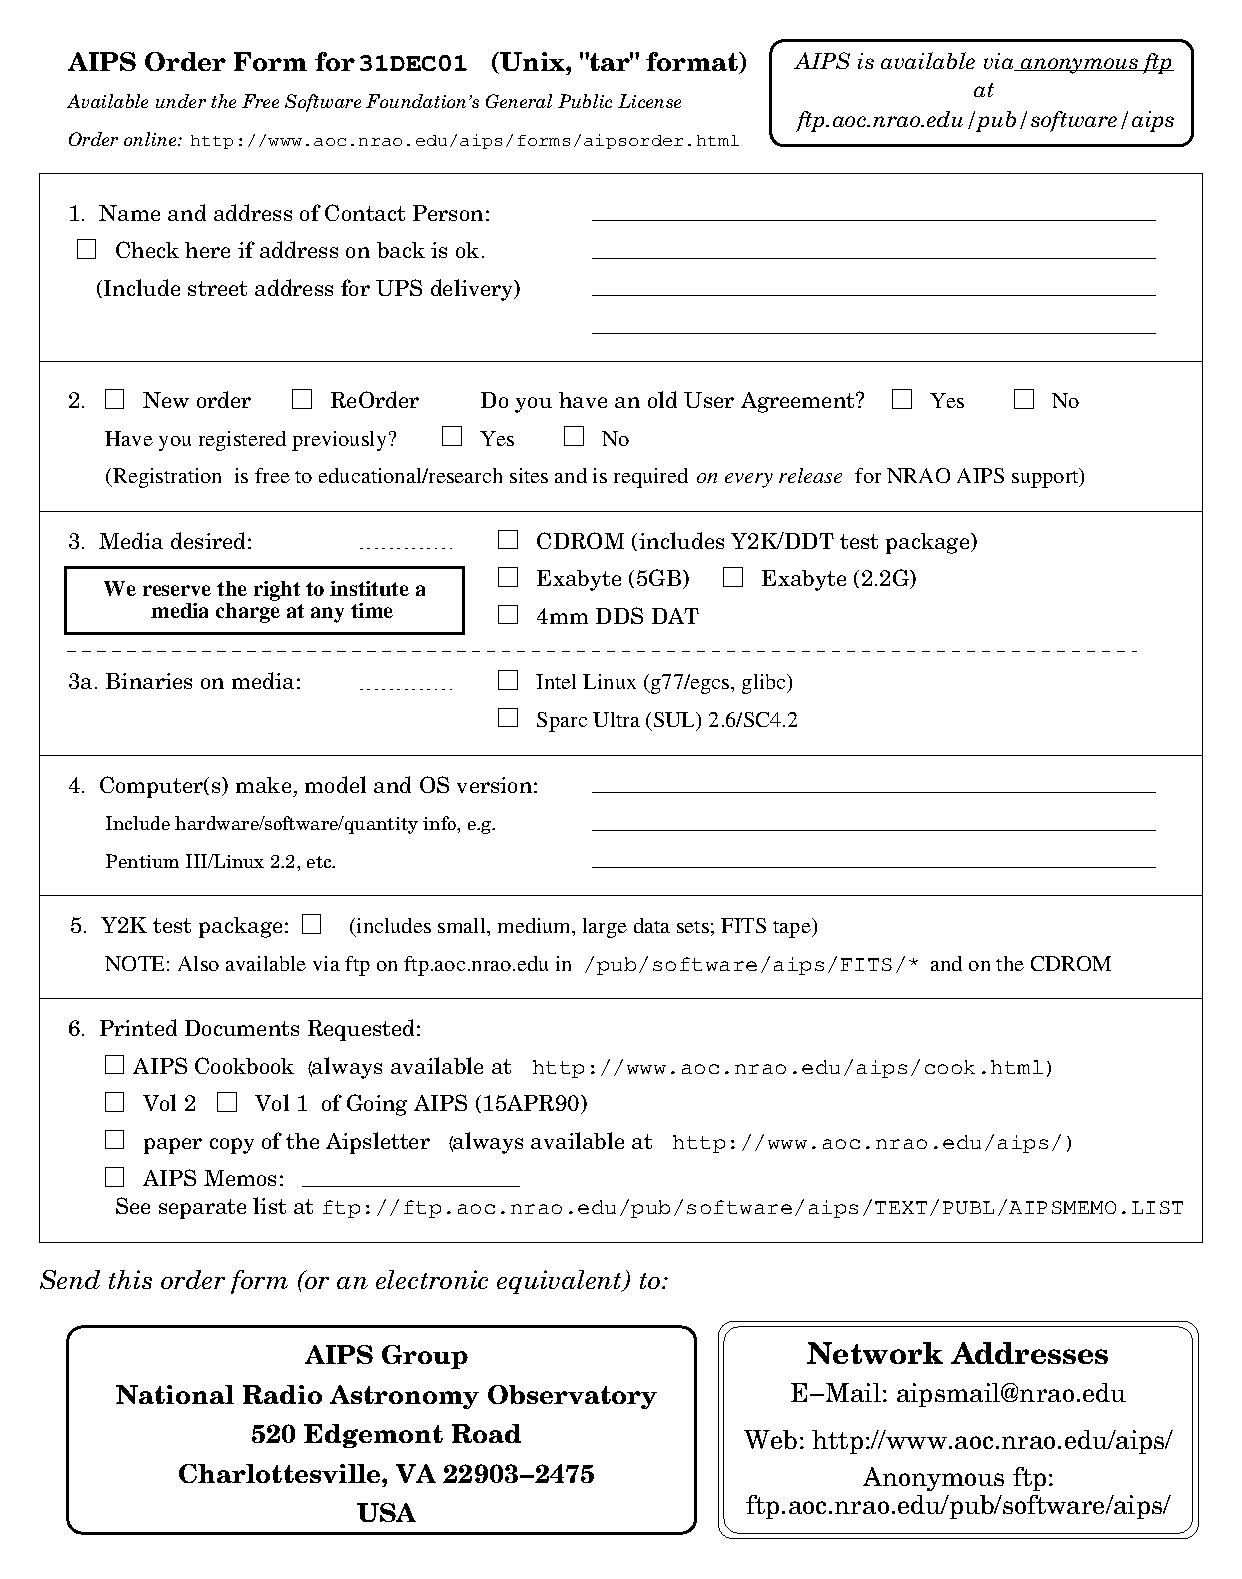
\includegraphics{FIG/AIPSORDER.PS}}}
%\vfill\eject
\vbox to 4.4in{
\vspace{12pt}
%\centerline{\rotatebox{-90}{\resizebox{!}{3.5in}{%
%\includegraphics{FIG/Mandrill.color.plt}}}}
\centerline{\resizebox{!}{3.5in}{\includegraphics{FIG/Mandrill.eps}}}
\vspace{12pt}
\centerline{{\huge \tt \AIPRELEASE}}
\vspace{12pt}
\vfill}
\phantom{...}
\centerline{\resizebox{!}{!}{\includegraphics{FIG/AIPSLETS.PS}}}

\end{document}
